\section{Uživateslká Příručka}

Tato sekce vás provede skrze různé funkcionality aplikace. Přeskočte na
podsekci, která vás zajímá.

\subsection{Přihlášení a registrace}

Po navigaci na adresu Memopadu jsou před Vámi tlačítka Přihlásit a Registrovat:

Pokud již účet máte, můžete vyplnit svoje údaje do polí username a password a
poté kliknout na tlačítko \uv{Login}.

Pokud účet ještě nemáte, klikněte na růžové tlačítko \uv{Register} a vyplňte
všechny pole. Po kliknutí na modré tlačítko \uv{Register} budete automaticky
přihlášeni.

Pokud jste nějakou náhodou skončili na obrazovce registra, ale účet už máte,
můžete kliknout na růžové tlačítko \uv{Login}, aby jste se vrátili na obrazovku
přihlášení.
\begin{figure}[h]
    \begin{minipage}[t]{0.45\textwidth}
        \begin{center}
            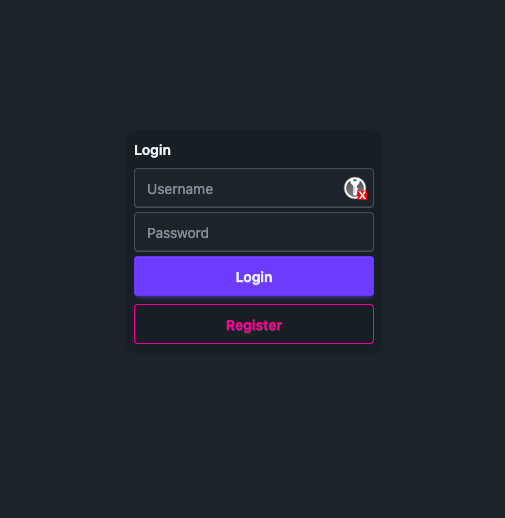
\includegraphics[width=0.9\linewidth]{graphics/login_screen.png}
            \caption{Obrazovka přihlášení}
            \label{fig:loginscreen}
        \end{center}
    \end{minipage}
    \hfill
    \begin{minipage}[t]{0.45\textwidth}
        \begin{center}
            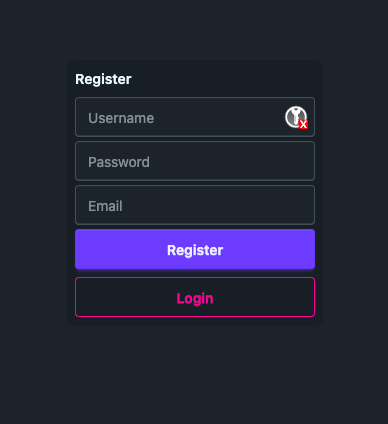
\includegraphics[width=0.9\linewidth]{graphics/register_screen.png}
            \caption{Obrazovka registrace}
            \label{fig:registerscreen}
        \end{center}
    \end{minipage}
\end{figure}

\subsection{Uživatelské Rozhraní}

Po přihlášení můžeme vidět uživatelské rozhraní MemoPadu. Následující grafika znázorňuje různé ovládací prvky rozhraní.

\begin{figure}[h]
    \begin{center}
        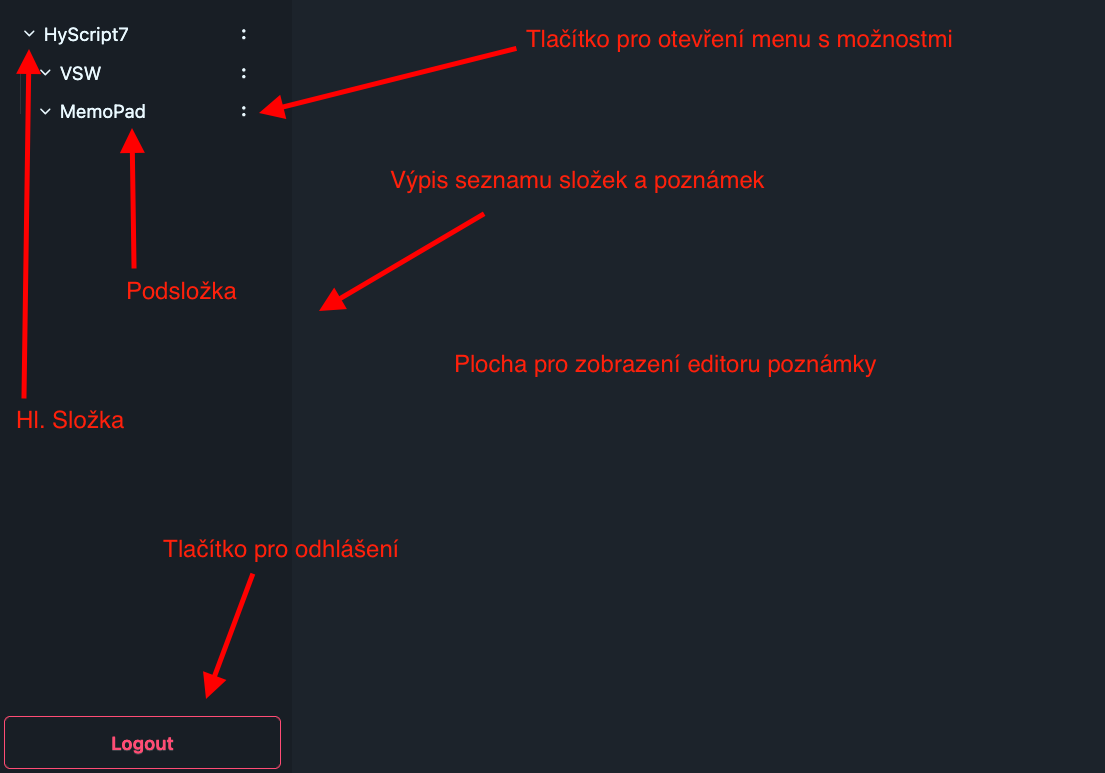
\includegraphics[width=0.5\linewidth]{graphics/ui.png}
        \caption{Uživatelské rozhraní MemoPadu}
        \label{fig:ui}
    \end{center}
\end{figure}
